%%%%%%%%%%%%%%%%%%%%%%%%%%%%%%%%%%%%%%%%%%%%%%%%%%%%%%%%%%%%%%%%%%%%%%%%%%%
%%                                                                       %%
%%     LaTeX + CTeX 《应用概率统计》论文模板, 只针对 A4 纸中文稿.        %%
%%                                                                       %%
%%%%%%%%%%%%%%%%%%%%%%%%%%%%%%%%%%%%%%%%%%%%%%%%%%%%%%%%%%%%%%%%%%%%%%%%%%%

%%%%%%%%%%%%%%%%%%%%%%%%%%%%%%%%%%%%%%%%%%%%%%%%%%%%%%%%%%%%%%%%
%            中文稿 文章模板:A4 纸, 五号字, 单列              %
%%%%%%%%%%%%%%%%%%%%%%%%%%%%%%%%%%%%%%%%%%%%%%%%%%%%%%%%%%%%%%%%
\documentclass[a4paper,c5size,onecolumn,twoside,cap,Chinese]{APSart}
\begin{document}

\setcounter{page}{1}

%%%%%%%%%%%%%%%%%%%%%%%%%%%%%%%%%%%%%%%%%%%%%%%%%%%%%%%%%%%%%%%%
%%------------------ 编辑部提供的信息 ------------------------%%
%%%%%%%%%%%%%%%%%%%%%%%%%%%%%%%%%%%%%%%%%%%%%%%%%%%%%%%%%%%%%%%%
\newcommand{\pubvol}{xx}         % 卷号
\newcommand{\enpubvol}{xx}       % 卷号
\newcommand{\pubno}{x}           % 期号
\newcommand{\enpubno}{x}         % 期号
\newcommand{\pubyear}{20xx}      % 出版年份
\newcommand{\enpubyear}{20xx}    % 出版年份
\newcommand{\pubmonth}{xx}       % 出版月份
\newcommand{\enpubmonth}{xx}     % 出版月份
\newcommand{\ksym}{xxx}          % 开始页码
\newcommand{\jsym}{xxx}          % 结束页码
\newcommand{\receivedate}{本文XXXX年XX月XX日收到} % 论文收到日期
\newcommand{\modifydate}{XXXX年XX月XX日收到修改稿}% 论文修改日期
\newcommand{\doino}{10.3969/j.issn.1001-4268.20xx.0x.0xx} % doi号
%%
%%%%%%%%%%%%%%%%%%%%%%%%%%%%%%%%%%%%%%%%%%%%%%%%%%%%%%%%%%%%%%%%
%%-------------------- 作者提供的信息 ------------------------%%
%%%%%%%%%%%%%%%%%%%%%%%%%%%%%%%%%%%%%%%%%%%%%%%%%%%%%%%%%%%%%%%%
\newcommand{\runcnauthors}{第一作者姓名, 第二作者姓名} %超过两个作者的请用:第一作者姓名~等
\newcommand{\cnfirstauthor}{第一作者姓名}
\newcommand{\cnsecondauthor}{第二作者姓名}
\newcommand{\cnfirstinst}{第一作者单位(到部门), 省市, 邮政编码}
\newcommand{\cnsecondinst}{第二作者单位(到部门),省市, 邮政编码}
\newcommand{\cntitle}{论文题目}
\newcommand{\cnkeywords}{关键词1; 关键词2; ......}
\newcommand{\cnclassno}{O212.xx} % 中图分类号
%%
\newcommand{\enfirstauthor}{FIRST Name}
\newcommand{\ensecondauthor}{SECOND Name}
\newcommand{\enfirstinst}{First Author's Working Unit $($Up to Department$)$, Province, 
Zip Code, China}
\newcommand{\ensecondinst}{Second Author's Working Unit $($Up to Department$)$, Province, 
Zip Code, China}
\newcommand{\entitle}{English Title}
\newcommand{\enkeywords}{keyword 1; keyword 2; ......}
\newcommand{\amsno}{62Nxx} % AMS Subject Claassification
%%
%% 中文摘要
\newcommand{\cnabstract}{摘要内容.}
%% 英文摘要
\newcommand{\enabstract}{The abstract comes here.}
\newcommand{\fundinfo}{XXXX基金资助(12345678).}
\newcommand{\authorsinfo}{\textbf{作者信息}:~
第一作者(出生时间--),~性别,~职称,~主要研究方向:~xxxxxx,~E-mail:xxxxx@xxxx.xxx.xx~;
第二作者(出生时间--):~性别, 职称,主要研究方向:~xxxxxx,~E-mail:xxxxx@xxxx.xxx.xx~.}

%%%%%%%%%%%%%%%%%%%%%%%%%%%%%%%%%%%%%%%%%%%%%%%%%%%%%%%%%%%%%%%%
%        文章正文                                              %
%%%%%%%%%%%%%%%%%%%%%%%%%%%%%%%%%%%%%%%%%%%%%%%%%%%%%%%%%%%%%%%%

\title{\zihao{3}\bf{\cntitle}
\thanks{\scriptsize{\fundinfo}}
}
%%%%%%%%%%%%%%%%%%%%%%%%%%%%%%%%%%%%%%%%%%%%%%%%%%%%%%%%%%%%%%%%
% 作者姓名与单位:三种形式中选一种
% 后面英文摘要中的名字和单位同样处理
% ---------------------
% 第一种形式: 单一作者
% ---------------------
%\author{\zihao{4}\fangsong{\cnfirstauthor}\\[-1pt]
%{\zihao{-5}(\cnfirstinst)}}

% ---------------------
% 第二种形式: 同一单位 多个作者 -- 名字左右并列,
% ---------------------
%\author{\zihao{4}\fangsong{\cnfirstauthor\hy\hy\hy\cnsecondauthor}\\[-1pt]
%{\zihao{-5}(\cnfirstinst)}}

% ---------------------
% 第三种形式: 不同单位 多个作者 -- 名字与单位上下并列
% ---------------------
\author{\zihao{4}\fangsong{\cnfirstauthor}\\[-1pt]
{\zihao{-5}(\cnfirstinst)}\and
\zihao{4}\fangsong{\cnsecondauthor}\\[-1pt]
{\zihao{-5}(\cnsecondinst)}}
%%%%%%%%%%%%%%%%%%%%%%%%%%%%%%%%%%%%%%%%%%%%%%%%%%%%%%%%%%%%%%%

\date{} % 这一行用来去掉默认的日期显示
\maketitle
\vspace{-6mm}
%%%%%%%%%%%%%%%%%%%%%%%%%%%%%%%%%%%%%%%%%%%%%%%%%%%%%%%%%%%%%%%%
%  中文摘要
%%%%%%%%%%%%%%%%%%%%%%%%%%%%%%%%%%%%%%%%%%%%%%%%%%%%%%%%%%%%%%%%
\begin{center}
\begin{minipage}[c]{14cm}
\zihao{-5}
\hspace{2\ccwd}\textbf{摘~~~要:}\quad\cnabstract\\
\mbox{}\hspace{2\ccwd}\textbf{关键词:}\quad\cnkeywords\\
\mbox{}\hspace{2\ccwd}\textbf{中图分类号:}\quad\cnclassno
\end{minipage}
\end{center}
\footnote[0]{\scriptsize{\receivedate, \modifydate.\\
\authorsinfo}}\vspace{-1em}
%
%%%%%%%%%%%%%%%%%%%%%%%%%%%%%%%%%%%%%%%%%%%%%%%%%%%%%%%%%%%%%%%%
%  正文由此开始
%%%%%%%%%%%%%%%%%%%%%%%%%%%%%%%%%%%%%%%%%%%%%%%%%%%%%%%%%%%%%%%%

%%%%%%%%%%%%%%%%%%%%%%%%%%%%%%%%%%%%%%%%%%%%%%%%%%%%%%%%%%%%%%%%
\section{引\hy\hy\hy 言}
%%%%%%%%%%%%%%%%%%%%%%%%%%%%%%%%%%%%%%%%%%%%%%%%%%%%%%%%%%%%%%%%

这是专门为《应用概率统计》定制的\LaTeX{}模板.

%%%%%%%%%%%%%%%%%%%%%%%%%%%%%%%%%%%%%%%%%%%%%%%%%%%%%%%%%%%%%%%%
\section{常用环境}
%%%%%%%%%%%%%%%%%%%%%%%%%%%%%%%%%%%%%%%%%%%%%%%%%%%%%%%%%%%%%%%%

\subsection{分类说明}

学术论文排版主要涉及公式、定理、图形、表格、参考文献等浮动环境的录入, 为查阅与应用方便, 此模板对它们进行了适当的调整, 现说明如下:
\begin{enumerate}\setlength{\itemsep}{-0.1ex}
\item 数学公式(equation等), 编号在右侧, 置于圆括号中, 使用单一的编号方式, 使用\verb|\eqref{}| 引用;
\item 图形(figure)与表格(table), 编号居中, 使用单一的编号方式, 使用\verb|\ref{}|引用;
\item 定理类, 包括定理(theorem)、引理(lemma)、推论(corollary)、命题(proposition)、公理(axmiom)、性质(property)、例子(example)、问题(question)、记号(notation)、注释(remark)等, 编号在左侧, 它们使用连续的单层编号, 引用由\verb|\ref{}|完成.
\item 参考文献, 编号在左侧, 置于方括号中, 使用单一的编号方式,有三种引用:
\begin{itemize}
\item 一般引用, 使用\verb|\ncite{}|引用;
\item 带附加信息引用, 使用\verb|\rcite{}|引用;
\item 上标形式引用, \verb|\ucite{}|引用.
\end{itemize}
\end{enumerate}

\subsection{使用示例}

这里给出了一些公式、表格、插图、定理及各类引用的例子, 仅供参考.
\begin{equation}\label{eq:1}
\left\{\begin{aligned}
          \pi&=3.141\cdots\\
     \sqrt{2}&=1.414\cdots
         \end{aligned} \right.
\end{equation}
\begin{align}
          \pi&=3.1415926\cdots\nonumber\\
            &\approx 3.14.
\end{align}

\begin{table}[htbp]
\centering\zihao{5}
{\caption{带水平及竖线的表格\label{table:1}}}
\vskip2mm
\begin{tabular}{r|l||c|rrr|c|c}
\hline
Positiion & 俱乐部 & 比赛 & W & T & L & Goals & Points \\ [0.5ex]
\hline\hline
1 & Amesville Rockets & 33 & 19 & 13 & 1 & 66:31& 51:15\\
2 & Borden Comets     & 33 & 18 & 9 & 6 &65:37 & 45:21\\ \hline
$\vdots$& $\vdots$    &&&&& &$\vdots$\\ \hline
17 & Quincy Giants    & 33 & 7 & 5 & 21 & 40:89 &19:47\\ \hline
18 & Arlson Regulars  & 33 & 3 & 11 &19 & 37:74 &17:49 \\ \hline
\end{tabular}
\end{table}

\begin{figure}[htbp]
\centering
\includegraphics[width=10cm,height=3cm]{figs/sin}
\caption{一个浮动图\label{fig:fig4}}
\end{figure}

\begin{figure}[htbp]
\begin{minipage}[t]{0.45\linewidth}
\centering
\includegraphics[width=6cm,height=3cm]{figs/sin}
\caption{这是第一个子图\label{fig:float2-1}}
\end{minipage}%
\hfill
\begin{minipage}[t]{0.5\linewidth}
\centering
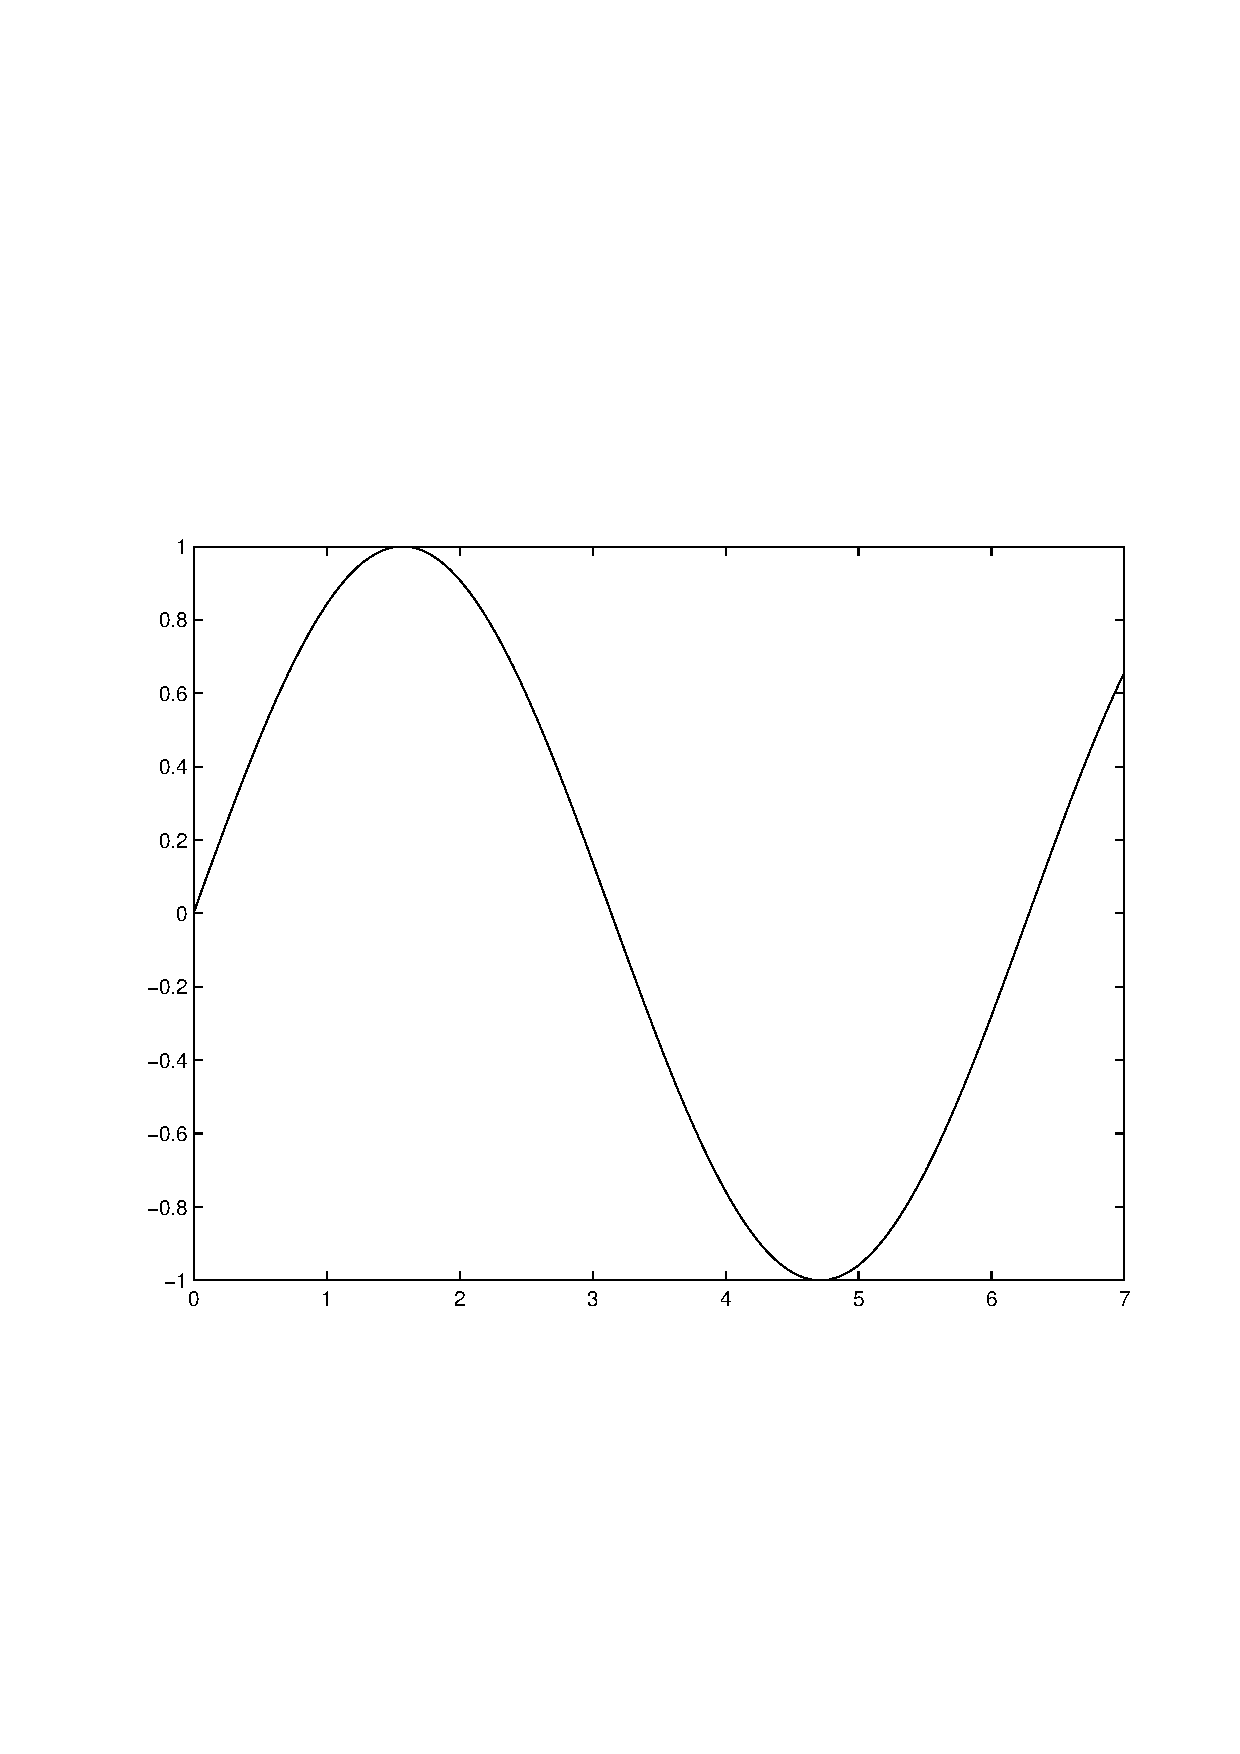
\includegraphics[width=5cm,height=3cm]{figs/fig}
\caption{这是第二个子图\label{fig:float2-2}}
\end{minipage}
\end{figure}

\begin{definition}
这是定义内容.
\end{definition}

\begin{lemma}
这是引理内容.
\end{lemma}

\begin{theorem}\label{thm-1}
这是定理\ref{thm-1}内容.
\end{theorem}

\begin{proof}
这是定理的证明.
\end{proof}

\begin{theorem}[唯一性定理]\label{thm-2}
这是定理\ref{thm-2}内容.
\end{theorem}

\begin{corollary}
这是推论.
\end{corollary}

\begin{proposition}
这是一个命题的内容.
\end{proposition}

下面是一些引用的例子:

\begin{example}
这里引用了第\pageref{eq:1}页的公式\eqref{eq:1}.
\end{example}

\begin{example}
这里引用了第\pageref{table:1}页的表格\ref{table:1}.
\end{example}

\begin{example}
这里引用了第\pageref{fig:float2-1}页的图形\ref{fig:float2-1}.
\end{example}

\begin{example}
这里引用了第\pageref{thm-1}页的定理\ref{thm-1}.
\end{example}

\begin{example}
这里引用了参考文献\ncite{Dengjs01}, 邓建松等\ucite{Dengjs01},
可能的变形有\rcite{Dengjs01}{第186页}, \rcite{Dengjs01}{第三章第2节定理2}.
\end{example}

\begin{example}
参考文献排版时``文章''的格式采用\ncite{Art}, ``书''的格式采用\ncite{Book}, 
``书中一个章节''的格式采用\ncite{Book-part}, `会议论文集''的格式采用\ncite{Conference}. 
参考文献按文中出现的先后次序编号.
\end{example}

%%%%%%%%%%%%%%%%%%%%%%%%%%%%%%%%%%%%%%%%%%%%%%%%%%%%%%%%%%%%%%%%
\section{特别说明}
%%%%%%%%%%%%%%%%%%%%%%%%%%%%%%%%%%%%%%%%%%%%%%%%%%%%%%%%%%%%%%%%

\begin{remark}
数学符号根据现有的规范重新进行了处理, 特别指出的有
\begin{itemize}
\item 数学中的花体字母应使用命令\verb|\mathscr{}|或缩略形式\verb|\scr{}|或重新定义的\verb|\cal{}|命令, 例如\verb|$\mathscr{A}, \scr{B}, \cal{C}$|分别产生$\mathscr{A}, \scr{B}, \cal{C}$.
\item 数学中的空心大写字体通常使用\verb|\mathbb{}|命令, 字体美观, 但对数字失效, 一种方案是使用宏包psfont的命令\verb|\mathds{}|,
    例如\verb|$\mathbb{A,B,R}, \mathbold{ABCP1}$|产生$\mathbb{A,B,R}$.
\item 数学中的黑体(大小写英文字母、数字、和希腊字母)可使用bm宏包中的命令\verb|\bm{}|. 若不使用宏包, 可将\verb|\bm|命令重新定义为
\begin{verbatim}
\newcommand{\bm}{\boldsymbol}
\end{verbatim}
\verb|\bm{2 Greeks $\alpha$, $\Gamma$}|产生2 Greeks $\bm{\alpha}$, $\bm{\Gamma}$.
\end{itemize}
\end{remark}

\begin{remark}
正确使用省略号: \verb|\dots|能智能识别省略号的位置.
\begin{verbatim}
$1+2+\cdots+n$; $i=1,2,\ldots,k$
$1+2+\dots+n$; $i=1,2,\dots,k$
\end{verbatim}
都得到$1+2+\dots+n$; $i=1,2,\dots,k$.
\end{remark}

\begin{remark}
数学函数应使用罗马正体, 使用\verb|\sin(x)|, \verb|\ln(y)|, \verb|\exp(z)|, \verb|\max|, \verb|\lim|, \verb|\sign(x)|分别产生$\sin(x)$, $\ln(y)$, $\exp(z)$, $\max$, $\lim$, $\sign(x)$. 概率$\pr$, 期望$\ep$, 方差$\var(x)$, 协方差$\cov(x,y)$分别由\verb|\pr|, \verb|\ep|, \verb|\var(x)|, \verb|\cov(x,y)|产生, 微分算子$\md$由\verb|\md|得到, 指数$\me$由\verb|\me|得到.
\end{remark}

\begin{remark}
正确使用定界符, 在此仅举一例:
\begin{verbatim}
$$
\frac{1+\bigl\{\,x\times[\,f(x)+g(x)\,]\,\bigr\}}{\sqrt{a+b}}2\biggm|_{x=0}
=\biggl(\,\frac{c}{a+b}\,\biggr)^{1/2}
$$
\end{verbatim}
$$
\frac{1+\bigl\{\,x\times[\,f(x)+g(x)\,]\,\bigr\}}{\sqrt{a+b}}2\biggm|_{x=0}
=\biggl(\,\frac{c}{a+b}\,\biggr)^{1/2}
$$
\end{remark}	

\begin{remark}
进一步学习和提高中英文\LaTeX 排版的水平、掌握一些特殊的技巧,
可参考文献\ncite{Dengjs01,Sangdy01,Chenzj02,Wangl2000,Huw2010,Lip04}.
\end{remark}

\vspace{6mm}
%%%%%%%%%%%%%%%%%%%%%%%%%%%%%%%%%%%%%%%%%%%%%%%%%%%%%%%%%%%%%%%%
%  参考文献
%%%%%%%%%%%%%%%%%%%%%%%%%%%%%%%%%%%%%%%%%%%%%%%%%%%%%%%%%%%%%%%%
\zihao{-5}
\begin{thebibliography}{99}
%\setlength{\parskip}{0pt}  %段落之间的竖直距离
\addtolength{\itemsep}{-0.8 em} % 缩小参考文献间的垂直间距
  \bibitem{Art} 作者. 文章题目[J]. {\kaishu 期刊名称}, 年份, {\bf 卷号(期数)}: 起始页码.
  \bibitem{Book} 作者. {\kaishu 书名}[M]. 出版地: 出版社, 年份.
  \bibitem{Book-part} 作者. {\kaishu 章节名}[M]// 编者. {\kaishu 书名}. 出版地: 出版社, 年份: 起始页码.
  \bibitem{Conference} 作者. 文章题目[C]// 编者. {\kaishu 会议论文集名}. 出版地: 出版社, 年份: 起始页码.
  \bibitem{Wangl2000} Reckdahl K. {\it Using Import graphics in \LaTeX2e}[M]. 王磊, 译. [出版地不详]: [出版社不详], 2000.
  \bibitem{Huw2010} 胡伟. {\kaishu \LaTeX{}2$\varepsilon$完全学习手册}[M]. 北京: 清华大学出版社, 2011.
  \bibitem{Lip04} 李平. {\kaishu \LaTeX{}2$\varepsilon$及常用宏包使用指南}[M], 北京: 清华大学出版社, 2004.
  \bibitem{Sangdy01} 桑大勇, 王瑛. {\kaishu 科技文献排版系统: \LaTeX 入门与提高}[M]. 武汉: 武汉大学出版社, 2001.
  \bibitem{Chenzj02} 陈志杰, 赵书钦, 万福永. {\kaishu \LaTeX{}入门与提高}[M]. 北京: 高等教育出版社, 2002.
  \bibitem{Dengjs01} 邓建松, 彭冉冉, 陈长松. {\kaishu \LaTeX{}2$\varepsilon$科技排版指南}[M]. 北京: 科学出版社, 2001.
\end{thebibliography}

%%%%%%%%%%%%%%%%%%%%%%%%%%%%%%%%%%%%%%%%%%%%%%%%%%%%%%%%%%%%%%%%
%  英文摘要
%%%%%%%%%%%%%%%%%%%%%%%%%%%%%%%%%%%%%%%%%%%%%%%%%%%%%%%%%%%%%%%%
\vspace{6mm}\hspace{-8mm}
\parbox{\textwidth}{
\begin{center}
\Large{\bf{\entitle}}\\[1em]
\textrm{\zihao{-4}\enfirstauthor}\\[0.2em]
\zihao{-5}(\textit{\enfirstinst})\\[0.8em]
\textrm{\zihao{-4}\ensecondauthor}\\[0.2em]
\zihao{-5}(\textit{\ensecondinst})
\end{center}

\mbox{}\hspace{2em}\textbf{Abstract:}\quad\enabstract\\
\mbox{}\hspace{2em}\textbf{Keywords:}\quad\enkeywords\\
\mbox{}\hspace{2em}\textbf{2010 Mathematics Subject Classification:}\quad\amsno}

%%%%%%%%%%%%%%%%%%%%%%%%%%%%%%%%%%%%%%%%%%%%%%%%%%%%%%%%%%%%%%%%
%  文章结束
%%%%%%%%%%%%%%%%%%%%%%%%%%%%%%%%%%%%%%%%%%%%%%%%%%%%%%%%%%%%%%%%
\clearpage
\end{document}
